%%%%%%%%%%%%%%%%%%%%%%%%%%%%%%%%%%%%%%%%%
% Beamer Presentation
% LaTeX Template
% Version 1.0 (10/11/12)
%
% This template has been downloaded from:
% http://www.LaTeXTemplates.com
%
% License:
% CC BY-NC-SA 3.0 (http://creativecommons.org/licenses/by-nc-sa/3.0/)
%
%%%%%%%%%%%%%%%%%%%%%%%%%%%%%%%%%%%%%%%%%

%----------------------------------------------------------------------------------------
%	PACKAGES AND THEMES
%----------------------------------------------------------------------------------------

\documentclass{beamer}

\mode<presentation> {

% The Beamer class comes with a number of default slide themes
% which change the colors and layouts of slides. Below this is a list
% of all the themes, uncomment each in turn to see what they look like.

%\usetheme{default}
%\usetheme{AnnArbor}
%\usetheme{Antibes}
%\usetheme{Bergen}
%\usetheme{Berkeley}
%\usetheme{Berlin}
%\usetheme{Boadilla}
%\usetheme{CambridgeUS}
\usetheme{Copenhagen}
%\usetheme{Darmstadt}
%\usetheme{Dresden}
%\usetheme{Frankfurt}
%\usetheme{Goettingen}
%\usetheme{Hannover}
%\usetheme{Ilmenau}
%\usetheme{JuanLesPins}
%\usetheme{Luebeck}
%\usetheme{Madrid}
%\usetheme{Malmoe}
%\usetheme{Marburg}
%\usetheme{Montpellier}
%\usetheme{PaloAlto}
%\usetheme{Pittsburgh}
%\usetheme{Rochester}
%\usetheme{Singapore}
%\usetheme{Szeged}
%\usetheme{Warsaw}

% As well as themes, the Beamer class has a number of color themes
% for any slide theme. Uncomment each of these in turn to see how it
% changes the colors of your current slide theme.

%\usecolortheme{albatross}
%\usecolortheme{beaver}
%\usecolortheme{beetle}
%\usecolortheme{crane}
%\usecolortheme{dolphin}
%\usecolortheme{dove}
%\usecolortheme{fly}
%\usecolortheme{lily}
%\usecolortheme{orchid}
%\usecolortheme{rose}
%\usecolortheme{seagull}
%\usecolortheme{seahorse}
\usecolortheme{whale}
%\usecolortheme{wolverine}

%\setbeamertemplate{footline} % To remove the footer line in all slides uncomment this line
%\setbeamertemplate{footline}[page number] % To replace the footer line in all slides with a simple slide count uncomment this line

%\setbeamertemplate{navigation symbols}{} % To remove the navigation symbols from the bottom of all slides uncomment this line
}
\usepackage{pdfpages}
\usepackage{graphicx} % Allows including images
\usepackage{booktabs} % Allows the use of \toprule, \midrule and \bottomrule in tables
  \usepackage{tikz}
\def\firstcircle{(0,0) circle (1.5cm)}
\def\secondcircle{(60:2cm) circle (1.5cm)}
\def\thirdcircle{(0:2cm) circle (1.5cm)}

%----------------------------------------------------------------------------------------
%	TITLE PAGE
%----------------------------------------------------------------------------------------

\title[Digital Ag]{Digital Agriculture Spring 2021} % The short title appears at the bottom of every slide, the full title is only on the title page

\author{Thanos Gentimis} % Your name
\institute[LSU] % Your institution as it will appear on the bottom of every slide, may be shorthand to save space
{
Louisiana State University Ag. Center\\ % Your institution for the title page
\medskip
\textit{agentimis1@lsu.edu} % Your email address
}
\date{} % Date, can be changed to a custom date

\begin{document}

\begin{frame}
\titlepage % Print the title page as the first slide
\end{frame}

%\begin{frame}
%\frametitle{Overview} % Table of contents slide, comment this block out to remove it
%\tableofcontents % Throughout your presentation, if you choose to use \section{} and \subsection{} commands, these will automatically be printed on this slide as an overview of your presentation
%\end{frame}

%----------------------------------------------------------------------------------------
%	PRESENTATION SLIDES
%----------------------------------------------------------------------------------------

%------------------------------------------------
\section{Course At a Glance} % Sections can be created in order to organize your presentation into discrete blocks, all sections and subsections are automatically printed in the table of contents as an overview of the talk
%------------------------------------------------

%\subsection{Subsection Example} % A subsection can be created just before a set of slides with a common theme to further break down your presentation into chunks

\begin{frame}
\frametitle{Basic Information}
\begin{itemize}
\item Instructor: Thanos Gentimis
\item Lab Location: M.Woodin Hall 0044
\item Lab Time: MT 13:00-14:50
\item Office Hours: T 12:00-1:00, W 12:00-1:00 or by appointment (Friday)
\item Office Location: M.Woodin Hall 0053
\item Email agentimis1@lsu.edu
\end{itemize}


\end{frame}

%------------------------------------------------

\begin{frame}
\frametitle{Class Focus}
\begin{center}
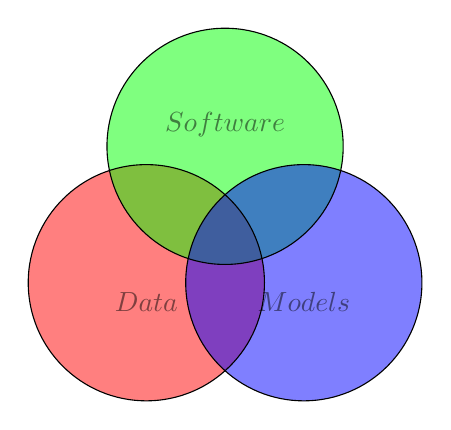
\begin{tikzpicture}
    \begin{scope}[fill opacity=0.5]
        \fill[red] \firstcircle;
        \fill[green] \secondcircle;
        \fill[blue] \thirdcircle;
        \draw \firstcircle node[below] {$Data $};
        \draw \secondcircle node [above] {$Software $};
        \draw \thirdcircle node [below] {$Models$};
    \end{scope}
\end{tikzpicture}
    \end{center}
\end{frame}

%------------------------------------------------
\section{Class Objectives}
\begin{frame}
\frametitle{Primary}
\begin{itemize}
\item<2-> Understand the complexities of data in Agriculture
\item<3-> Be able to collaborate with data analysts and other specialists
\item<4-> Create, enhance, update your research 

\end{itemize}

\end{frame}
%------------------------------------------------
\begin{frame}
\frametitle{Secondary}
\begin{itemize}
\item<2-> Understand basic modeling methods, especially machine learning
\item<3-> Get familiar with image processing
\item<4-> Be familiar with various relevant programs and computer languages
\end{itemize}

\end{frame}


\section{Basic Content}
%%------------------------------------------------
%\setbeamercolor{background canvas}{bg=}
%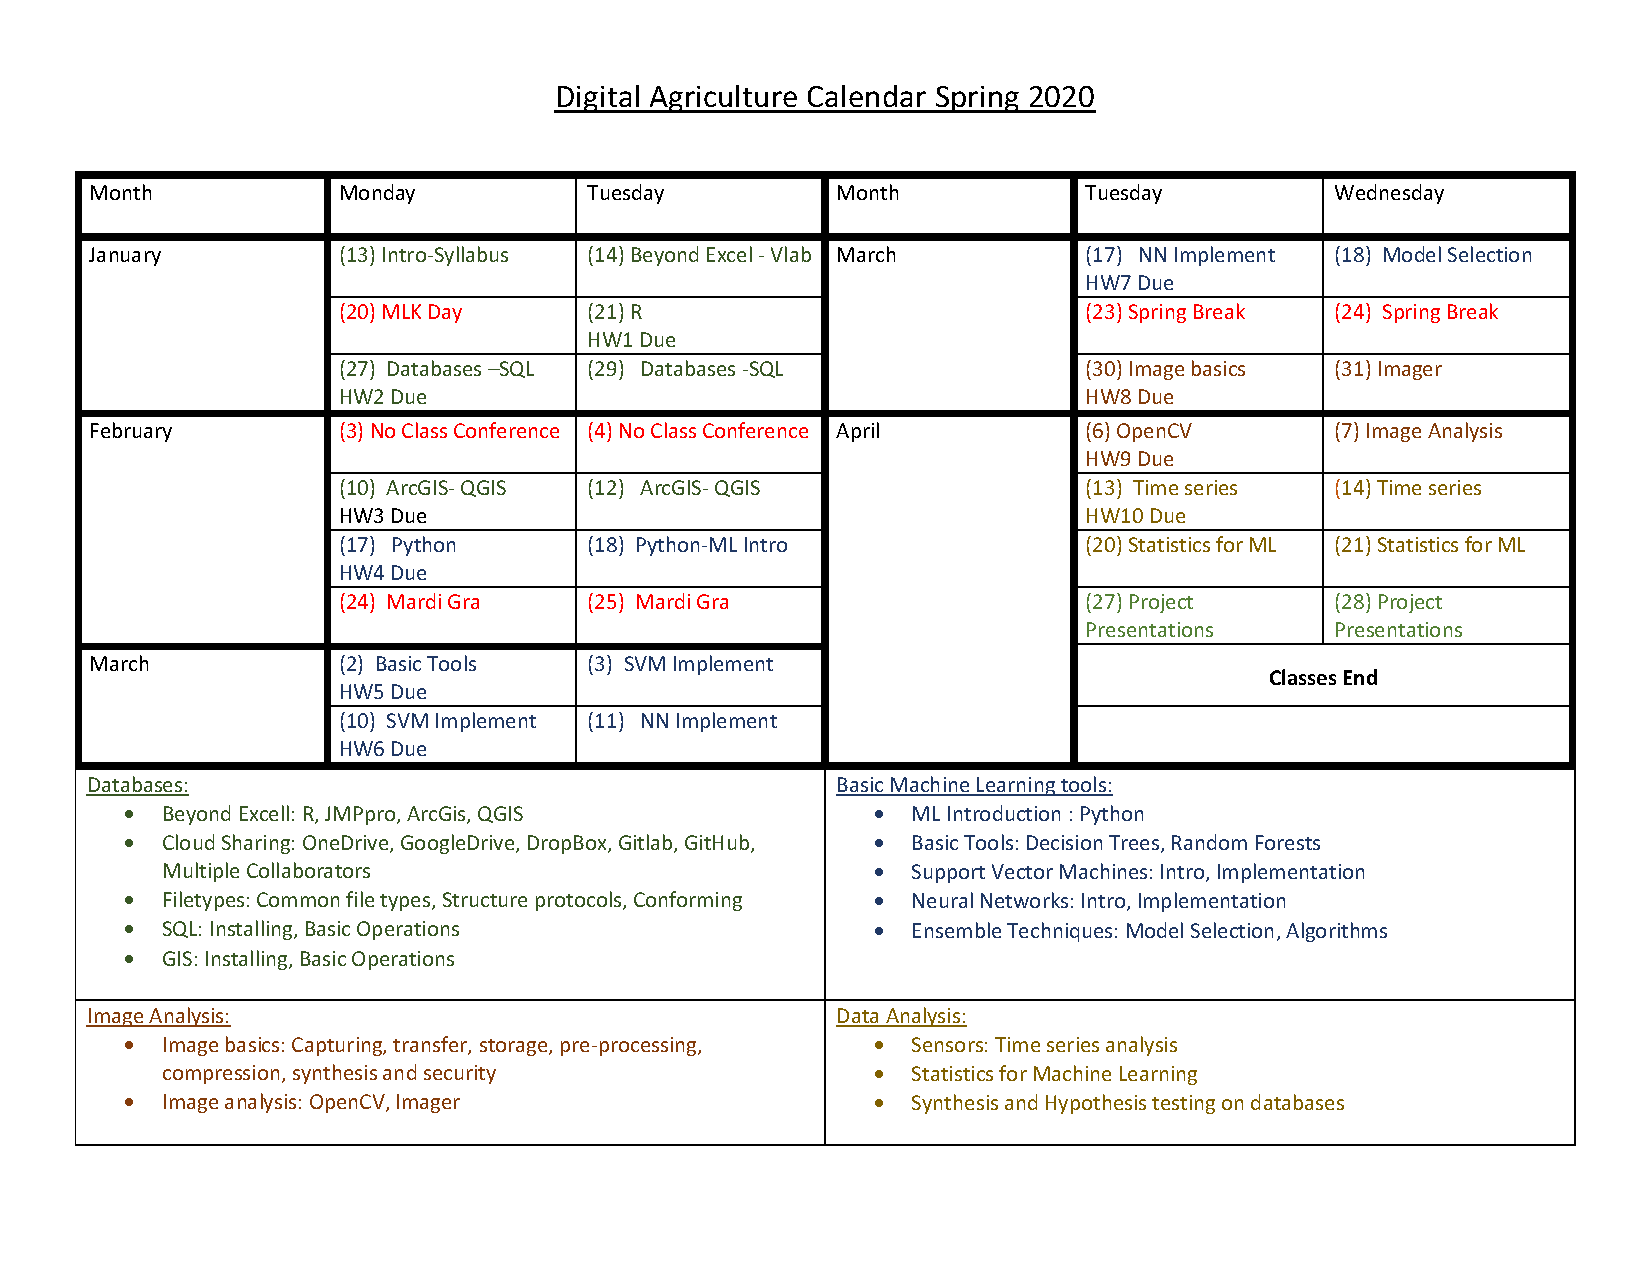
\includepdf{./Images/Calendar_2020_Spring.pdf}

%------------------------------------------------

\begin{frame}
\frametitle{Structured Data}



\begin{columns}[c] % The "c" option specifies centered vertical alignment while the "t" option is used for top vertical alignment
\begin{column}{0.5\textwidth}
\begin{enumerate}
\item Tables with numerical values
\item Structured Reports
\item Query based analyses
\end{enumerate}
\end{column}
\begin{column}{0.5\textwidth}

\begin{table}
\begin{tabular}{l l l}
\toprule
\textbf{Treatments} & \textbf{Response 1} \\
\midrule
Treatment 1 & 0.0003262 \\
Treatment 2 & 0.0015681 \\
Treatment 3 & 0.0009271 \\
\bottomrule
\end{tabular}
\end{table}
\end{column}
\end{columns}
\end{frame}

%------------------------------------------------

\begin{frame}
\frametitle{Time series}



\begin{columns}[c] % The "c" option specifies centered vertical alignment while the "t" option is used for top vertical alignment
\begin{column}{0.5\textwidth}
\begin{enumerate}
\item Functions of time
\item Trend analysis
\item Weather Data
\end{enumerate}
\end{column}
\begin{column}{0.5\textwidth}

\begin{figure}
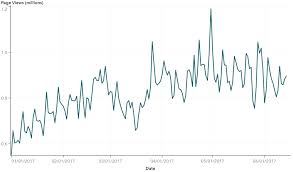
\includegraphics[scale=0.5]{./Images/time.jpg}
\end{figure}
\end{column}
\end{columns}
\end{frame}

%------------------------------------------------

\begin{frame}
\frametitle{Images}



\begin{columns}[c] % The "c" option specifies centered vertical alignment while the "t" option is used for top vertical alignment
\begin{column}{0.5\textwidth}
\begin{enumerate}
\item Drone Captured Images
\item Satellite Images
\item Geolocation 
\end{enumerate}
\end{column}
\begin{column}{0.5\textwidth}

\begin{figure}
\includegraphics[scale=0.03]{./Images/dgi.jpg}
\end{figure}
\end{column}
\end{columns}
\end{frame}

%------------------------------------------------
\begin{frame}
\frametitle{Software-Languages}

\begin{enumerate}
\item R
\item Python
\item ArcGis
\item QGis
\item Postgress (pgadmin)
\item JMPpro
 \end{enumerate}
\end{frame}

\begin{frame}
\frametitle{Cloud-Sharing}
\begin{enumerate}
\item Remote Servers
\item Googledrive
\item Gitlab
\item OneDrive
\end{enumerate}
\end{frame}

\begin{frame}
\frametitle{Requirements}

\begin{enumerate}
\item<2-> Outside of class work 
\item<3-> Open mind, patience 
\item<4-> Collaboration, team spirit, learn together
\item<5-> Ideas on improvement!
\end{enumerate}
\end{frame}
 
\begin{frame}
\frametitle{Grade}

\begin{enumerate}
\item<2-> 10 Homework, 8 of them count 5*8=40 points
\item<3-> 1 project, 60 points
\item<4-> Check syllabus for letter grades!
\end{enumerate}
\end{frame} 
 
 
\end{document}







